% @author Arian Helberg

\chapter{Konzepte}
Mit der Erstellung eines Programms zur Synthetisierung von Ähnlichkeitsabbildungen einer vom Benutzer
erstellten Verzweigungsstruktur soll die Praktibilität aktueller Forschungsansätze untersucht werden.
\\~\\
Folgende Kernkonzepte werden erläutert und umgesetzt:
\begin{itemize}
    \item Visualisierung und prozessorientiertes Erstellen von Basisstrukturen,
    \item Organisation in einer prozessoptimierten, baumähnlichen Topologie,
    \item L-System-Repräsentationen,
    \item Algorithmen zur Inferierung, Komprimierung, Generalisierung und
    \item Verarbeitung von Transformationsparametern
\end{itemize}

\section{Probleme \& Lösungsansätze}

\subsection*{Visualisierung}
Um eine geführte Erstellung der Basisstruktur zu ermöglichen, muss diese während der Erstellung sichtbar gemacht werden.
Hierzu werden die Templates in Form von Zeichenketten angelegt und mittels Turtle-Grafik visualisiert.
Eine Turtle-Grafik beschreibt die Interpretation einer Zeichenkette als Bild durch Ausführen eines Logo-Turtle-Algorithmus.
Weiter wird auch zur Evaluation von Ergebnissen eine Visualisierung benötigt.
Da die Verzweigungsstrukturen in L-System-Repräsentation vorliegen, wird hierzu eine Interpretationsfunktion benötigt,
die diese Ersetzungssysteme in Bildform darstellen.
Ein L-System wird durch Ausführung in eine erweiterte Zeichenkette überführt und als Turtle-Grafik beschrieben
~\cite{prusinkiewicz_1986}.

\subsection*{Basisstruktur}
Der Benutzer nutzt grafische Bendienelemente, um eingelesene Templates auszuwählen, Transformationsparameter anzupassen
und um anschließend die Instanzen der Basisstruktur hinzuzufügen.
Im Folgenden wird diese Basisstruktur u.a. Grundstruktur und Eingabestruktur genannt.

\subsection*{Baumstruktur}
Um Grundstrukturen mittels verschiedener Algorithmen untersuchen zu können, werden die einzelnen Template-Instanzen in
einer baumähnlichen Struktur organisiert.
Transformationsparameter einer Instanz beschreiben die räumlichen Veränderung gegenüber des zugrundeliegenden Templates
und haben daher keine Aussagekraft in Bezug auf die Strukturtopologie der Basisstruktur.
Diese Arbeit fokussiert sich auf topologische Eigenschaften von Verzweigungsstrukturen (z.B. Rekursionen).
Darum bilden die einzelnen Template-Instanzen die Knoten der Baumtopologie, während die Kanten die räumlichen Transformationen
darstellen.
So wird eine datenstrukturelle Trennung zwischen Topologie und räumlichen Transformationen geschaffen.
Diese baumähnliche Struktur ist ispiriert durch~\cite{guo_2020}, Kapitel 4.2 \textit{Grammar inference}

\subsection*{Inferieren}
Das Smallest Grammar Problem, also das Finden der kleinsten, kontextfreien Grammatik, welche eine bestimmte Zeichenkette
generiert, ist ein offenes Problem der Informatik mit einem Annäherungsverhältnis von weniger als $\frac{8569}{8568}$
(NP-hard).
Primär wird in der Forschung nach Algorithmen gesucht, die ein akzeptables Ergebnis liefern.
In dieser Arbeit wird ein Algorithmus präsentiert, der die Knoten der Baumstruktur in einzelne Symbole umwandelt, mit
Produktionregeln verknüpft und diese dem resultierenden L-System hinzufügt.
Dieses L-System repräsentiert lediglich die Eingabestruktur.

\newpage

\subsection*{Komprimieren}
Um ein kompaktes, gewichtetes L-System zu erzeugen, werden sich wiederholende Unterrbäume gesucht und ersetzt.
Eine Gewichtung wird angewendet, um das zu erzeugende L-System mit kleiner Regelmenge oder mit
großer Regelmenge auszustatten.
Eine Kostenfunktion stellt hierbei die Anzahl Symbole aller RHS der Produktionsregeln mit der Menge an Anwendungen der
LHS gegenüber.

\subsection*{Generalisieren}
Da das kompakte L-System eine Repräsentation der vom Benutzer erzeugten Verzweigungsstruktur darstellt, werden ähnliche
Regeln miteinander verbunden (Merge) und mit einer Wahrscheinlichkeit versehen, um nicht-deterministische Regeln hinzuzufügen.
Eine weitere Kostenfunktion bewertet den Merge zweier Produktionregeln und wendet eine Gewichtung über die Länge der Grammatik
zur Änderungsdistanz der alten (ohne Merge) zur neuen Grammatik um.

\subsection*{Transformationen}
Die vom Benutzer vergeben Werte der Transformationsparameter werden während der Erstellung der Eingabestruktur in
einer Häufigkietsverteilung organisiert und bei Ausführung des generalisierten L-Systems angewendet.
So werden Transformationen nach ihrer statistischen Häufigkeit angewendet.

\newpage

\section{Workflows \& Algorithmen}
\label{algo}

\subsubsection*{Verzweigungsstruktur erstellen}
Um als Benutzer des Systems eine Verzweigungsstruktur zu erstellen, wird folgender Arbeitsablauf umgesetzt:
\begin{algorithm}[caption={Erstellen einer Verzweigungsstruktur}, label={alg1}]
    Erster Anker ist vorselektiert
    Wiederhole, bis Struktur fertiggestellt ist:
        Selektiere ein Template aus der Liste
        Setzte Parameter
        Bestätige Auswahl und Parameter
        Zeichne ausgewähltes Template mit Parametern
        Wähle nächsten Anker aus
\end{algorithm}

\subsubsection*{L-System inferieren}
Aus der Verzweigungsstruktur kann nun ein L-System erzeugt werden.
Hierzu wird ein neuer Algorithmus (siehe Algorithmus 32) präsentiert:\\~\\
Zunächst werden L-System-Komponenten initialisiert (Zeile 2-6) für $\mathcal{L}=\langle M,\omega,R \rangle$:
\begin{itemize}
    \item Das Alphabet wird mit den Sybolen F und S initialisiert, da F als Repräsentation einer grundlegenden
    Zeichenoperation und S als Axiom in jeder Anwendung des Algorithmus vorkommt
    \item Die erste Produktionsregel $\alpha$ umfasst die Abbildung des Axioms auf einen neues Symbol, das nicht im Alphabet
    vorkommt. Das Alphabet wird stets um ein Symbol lexikografischer Ordnung ergänzt
    \begin{itemize}
        \item Bsp.: $\{A,B,C\}$ wird ein neues, unbekanntes Symbol hinzugefügt $\rightarrow \{A,B,C,D\}$
    \end{itemize}
    \item Die Variable $\beta$ hält zu untersuchende Knoten der Baumtopologie, welche nach Breitensuche iteriert werden.
    Die erste Iteration startet bei Wurzelknoten S.
    \item Als letzten Schritt der Initialisierung wird dem Alphabet ein neues Symbol hinzugefügt, das durch die Variable
    $\gamma$ gehalten wird.
\end{itemize}
Die Schleife des Algorithmus beschäftigt sich mit der Iterierung des Baumes und dem Erstellen neuer Symbole und
Produktionsregeln für das resultierende L-Systems (Zeile 8-17):
\begin{itemize}
    \item Die in den Knoten des Baumes gehaltenen Template-Instanzen entprechen einer Zeichenkette, die durch eine
    Turtle-Grafik interpretiert, einem vom Benutzer transformierten Tempalte entspricht. Diese Zeichenkette wird in
    $\delta$ gespeichert
    \item In Zeile 9-12 wird die genannte Zeichenkette auf Verzweiungsvariablen ($A-Z$; $F$ ausgeschlossen) untersucht.
    Diese werden durch ein neues Symbol, das dem Alphabet hinzugefügt wird, ersetzt. Anschließend wird eine Produktionregel,
    die auf die veränderte Zeichenkette abbilded, der Produktionsregelmenge hinzugefügt.
    \item Zeile 13 prüft, ob es Symbol im Alphabet gibt, das nicht als Ziel einer Produktionregel in der Produktionsregelmenge
    definiert ist. Ist dies der Fall, wird dieses als Ziel der nächsten Produktion gesetzt. Andernfalls schließt der
    Algorithmus ab
    \item Schleifen-Attribut ist hier das Setzen des nächsten Knotens am Ende der Schleife (Zeile 17)
\end{itemize}

\begin{algorithm}[caption={Inferieren eines L-Systems aus einer Baumstruktur}, label={alg2}]
    Initialisierung:
        $M=\{F,S\}$
        $\omega=S$
        $R \gets \{\alpha$: $S \rightarrow A\}$
        $\beta=$ nächster Knoten
        $M \gets \gamma \in \{A,B,\dots,Z\}$, mit $\gamma \notin M$
    Schleife:
        $\delta=$ Wort von $\beta$
        $\forall \{A,B,\dots,Z\} \setminus F \in \delta:$
        Ersetze mit $\zeta \in \{A,B,\dots,Z\}$, mit $\zeta \notin M$
        $M \gets \zeta$
        $R \gets \{\gamma\rightarrow\delta\}$
        Wenn es ein Symbol $\eta$ in $M\setminus\{F,S\}$ gibt mit $\{\eta \rightarrow bel.\} \notin R$:
            $\gamma=\eta$
        Sonst:
            Breche Schleife ab
        $\beta=$ nächster Knoten
\end{algorithm}

\subsubsection*{L-System komprimieren}
\citeauthor{guo_2020} führt einen Algorithmus zum Inferieren einer Grammatik aus einer Baumstruktur ein~\cite{guo_2020}.
Zum Einen wird ein L-System aufgebaut, zum Andern die Baumtopologie durch Finden maximaler Subbäume reduziert.
Die Reduktion wird im folgenden Algorithmus 33 adaptiert:\\~\\
Initialisierung (Zeile 2-5):
\begin{itemize}
    \item Das L-System, welches der Eingabe des Algorithmus entspricht, wird ausgeführt und
    die resultierende Zeichenkette wird in $\mathcal{L^+}$ gespeichert
    \item Ein Gewichtungsparameter $w_l$ wird eingeführt, der eine Kostenfunktion (Zeile 11) nach Anzahl an Symbolen
    der RHS von Produktionsregeln und Anzahl deren Anwendung gewichten soll.
    \item Anschließend wird ein maximaler Subbaum durch geschachtelte Iteration des Baumes $T$ gesucht und als $T'$ gesetzt
    \item Es werden ausschließlich maximale Unterbäume behandelt, die mindestens zwei mal im Baum vorkommen
\end{itemize}
Die Schleife (Zeile 7-13) stellt die Reduzierung dar:
\begin{itemize}
    \item Zunächst werden alle Vorkommen des maximalen Unterbaumes durch ein neues Symbol ersetzt
    \item Aus diesem Subbaum wird ein L-System inferriert, das wiederum in eine erweiterte Zeichenkette ausgeführt wird
    \item Die Zeichenkette wird als LHS einer neuen Produktionsregel gesetzt, die auf das neue Symbel abzielt
    \item Das alte L-System kann nun mit dem veränderten L-System mittels Kostenfunktion verglichen werden (Zeile 9):
    Liegen die Kosten des veränderten L-Systems unter den Kosten des Alten, wird die Reduktion beendet.
    Andernfalls gilt der Subbaum nun als Eingabebaum und das veränderte Ersetzungssystem als Eingabe-L-System
\end{itemize}

\begin{algorithm}[caption={Erstellen eines kompakten L-Systems mit Gewichtung $w_l$}, label={alg3}]
Initialisierung:
    $\mathcal{L}^+ \leftarrow L_s$
    $\mathcal{L}=\emptyset$
    Setze Gewichtungsparameter $w_l \in [0,1]$
    Finde maximalen Unterbaum $T'$ aus $T$ mit Wiederholungen $n>1$
Schleife (Reduzierung):
    Ersetze alle Vorkommen von $T'$ mit dem selben Symbol $\gamma \in \{A,B,\dots,Z\}$
    $R \leftarrow \{\gamma \rightarrow L_s\}$ mit $L_s$ aus $T'$, $R$ aus $\mathcal{L}$
    Wenn $C_i(\mathcal{L}) \geq C_i(\mathcal{L}^+)$:
        Breche Schleife ab
    $T \leftarrow T'$
    $\mathcal{L}^+ \leftarrow \mathcal{L}$
    Finde maximalen Unterbaum $T'$ aus $T$ mit Wiederholungen $n>1$
\end{algorithm}

\begin{algorithm}[caption={Kostenfunktion $C_i$ mit Gewichtung $w_l$}, label={alg4}]
$C_i(\mathcal{L})= \sum\limits_{A(P) \rightarrow M^* \in \mathcal{L}} w_l * |M^*| + (1 - w_l) * N(A(P)\rightarrow M^*)$
\end{algorithm}
mit $N(\cdot)$ als Zählfunktion für die Anzahl Wiederholungen einer \textit{LHS} einer Regel in einem
ausgeführten L-System.

\subsubsection*{L-System generalisieren}
Da das kompakte L-System eine Repräsentation der vom Benutzer erzeugten Verzweigungsstruktur darstellt, werden
nun ähnliche Regeln miteinander verbunden und mit einer Wahrscheinlichkeit versehen, um nicht-deterministische
Regeln hinzuzufügen.
Sowohl Längenfunktionen, Kostenfunktionen und Distanzalgorithmen, als auch der Grundalgorithmus sind aus ~\cite{guo_2020}
entnommen und bauen sich wie folgt auf:

\begin{itemize}
    \item Die Längenfunktion $L$, die auf eine Grammatik angewendet wird, summiert die Anzahl Symbole des Alphabets mit
    der Anzahl an RHS der Produktionsregeln und misst somit die Gesamtheit aller Symbole, die das L-System abbilden soll
    (Länge der Grammatik)
    \item Der Abstand zweier Zeichenketten kann mit der \textit{String Edit Distance} ermittelt werden. Diese wird über
    die Funktion $D_s$ abgebildet. Hierbei wird die Anzahl an Operationen summiert, die für die Überführung einer Zeichenkette
    in eine Andere nötig sind (Zeichenkettenaustausch, -einschub und -löschung)
    \item Mit $D_s$ kann nun auch der Abstand zweier Grammatiken zueinander bestimmt werden. Diese Funktion wird mit
    $D_g$ abgebildet
    \item Die Kostenfunktion $C_g$ nutzt die Länge und Distanz von Grammatiken, um Kosten einer Überführung einer Grammatik
    in eine andere messen zu können. Sie berechnet also sie die Kosten, um $L^*$ in $L^+$ zu überführen.
    Der Parameter $w_0$ gewichtet hierbei die Differenz der Länge der Grammatiken und die Anzahl Operationen, die zur
    Überführung nötig sind. Die Überführungskosten werden in der Variable $C^{old}_g$ zur Verfügung gestellt.
\end{itemize}

\begin{algorithm}[caption={Längenfunktion $L$ für Grammatiken}]
$L(\mathcal{L}) = |M| + \sum\limits_{A(P) \rightarrow M^* \in \mathcal{L}} |M^*|$
\end{algorithm}

\begin{algorithm}[caption={Grammar Edit Distance}]
$D_g(\mathcal{L}^+, \mathcal{L}^*)= \sum\limits_{(A(P) \rightarrow M^*_A , B(P) \rightarrow M^*_B) \in M(\mathcal{L^+} \rightarrow \mathcal{L^*})} D_s(M^*_A, M^*_B)$
\end{algorithm}

\begin{algorithm}[caption={Kostenfunktion $C_g$ mit Gewichtung $w_0$}]
$C_g(\mathcal{L}^*, \mathcal{L}^+) = w_0 * (L(\mathcal{L}^*) - L(\mathcal{L}^+)) + (1 - w_0) + D_g(\mathcal{L}^+, \mathcal{L}^*)$
\end{algorithm}

\newpage

Algorithmus 38 zum Generalisieren eines L-Systems:\\~\\
Initialisierung (Zeile 2-4):
\begin{itemize}
    \item Das zu untersuchendes Tuple bestehend aus zwei Produktionsregeln (Regelpaar) und wird in der Variable $p^*$ gehalten
    \item L-Systeme, die sich infolge eines Merges geändert haben, werden in $L^+$ und Eingabe-L-systeme in $L^*$ gespeichert
\end{itemize}
Generalisierung (Zeile 6-13):
\begin{itemize}
    \item $\mathcal{P}$ ist die Menge aller möglichen Regelpaare aus $L^*$
    \item Das Regelpaar, das beim Merge die geringsten Kosten für die Überführung in die neue Grammatik aufweist, wird in
    $p^*$ gehalten
    \item Sind diese Kosten positiv, wird die Generalisierung abgebrochen
    \item Andernfalls werden die Variablen $c^*$ als Delta-Kosten, $C^{old}_g$ und $L^*$ entsprechen gesetzt
    \item Sollte die Differenz der Überführungskosten positiv sein, wird die Generalisierung abgebrochen
\end{itemize}

\begin{algorithm}[caption={Generalisieren eines L-Systems mit Gewichtung $w_0$}]
Initialisierung:
    Regelpaar $p^* = \emptyset$
    $\mathcal{L}^* = \mathcal{L}^+$
    $C_g^{old} = C_g(\mathcal{L}^* + \{p^*\}, \mathcal{L}^*)$
Schleife:
    Finde Regelpaar $p^*$ mit minimalen Kosten $C_g(\mathcal{L}^* + \{p_i\}, \mathcal{L}^*), \forall p_i \in \mathcal{P}$
    Wenn $C_g(\mathcal{L}^* + \{p^*\}, \mathcal{L}^*) \geq 0$:
        Breche Schleife ab
    $c^* = C_g(\mathcal{L}^* + \{p^*\}, \mathcal{L}^*) - C_g^{old}$
    $C_g^{old} = C_g(\mathcal{L}^* + \{p^*\}, \mathcal{L}^*)$
    $\mathcal{L}^* = \mathcal{L}^* + \{p^*\}$
    Wenn $c^* > 0$:
        Breche Schleife ab
\end{algorithm}

\newpage

\section{Softwarearchitektur}
Die Gliederung der Inhalte für die Softwarearchitektur erfolgt nach der arc42-Vorlage~\cite{arc42}

\subsection*{Qualitätsziele}
Um die wesentlichen Features des Systems in einem Programm umzusetzen, werden folgende Qualitätsziele definiert,
priorisiert (absteigend) und umgesetzt:
\begin{itemize}
    \item \textbf{Funktionalität} durch Umsetzen aller Teilsysteme in Vollständigkeit, Korrektheit, Angemessenheit
    \item \textbf{Interoperabilität} durch Nutzen einer allgemeinen Repräsentation von L-Systemen, damit diese
    auch in anderen Programmen oder Algorithmen verwendet werden kann
    \item \textbf{Erweiterbarkeit} durch offene Entwurfsmuster (Design Patterns)
    \item \textbf{Modularität} durch Implementierung für effiziente Wartung und Erweiterung
    \item \textbf{Effizienz} durch effiziente Programmierung
    \item \textbf{Attraktivität} durch intuitive Benutzung (Benutzerfreundlichkeit)
    \item \textbf{Plattformunabhängigkeit} durch Verwenden des Java-Frameworks
\end{itemize}

\newpage

\subsection*{Kontextabgrenzung}
Die Systemgrenzen werden zum Einen durch die Interaktion mit dem Benutzer, zum Anderen durch die Interaktion mit
dem Dateisystem des Host-Systems und dem Zugreifen und Lesen der Template-Dateien definiert.
Hierbei wird die Erstellung der Basisstruktur als nicht-technische Interaktion und das Einlesen der Dateien als
technische Interaktion gesehen.
\begin{figure}[H]
    \centering
    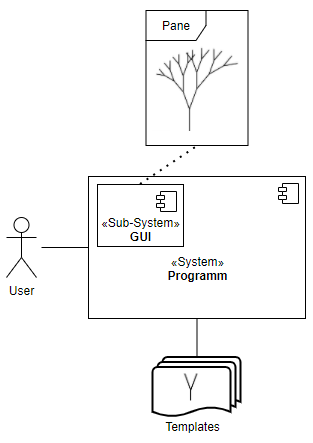
\includegraphics[width=6.2cm]{../images/Fachlicher_Kontext.PNG}
    \caption{System und Systemumgebung}
\end{figure}
\begin{figure}[H]
    \centering
    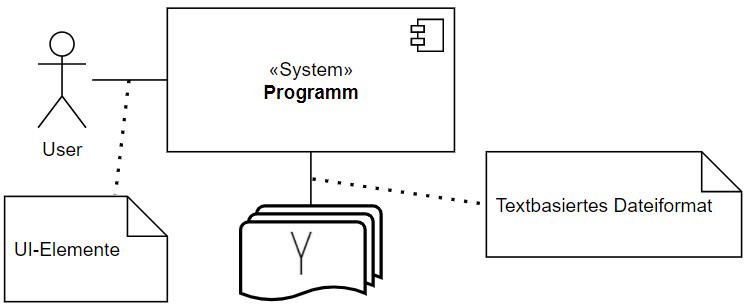
\includegraphics[width=10cm]{../images/Technischer_Kontext.PNG}
    \caption{Interaktion zwischen System und Systemumgebung}
\end{figure}

\subsection*{Lösungsstrategie}
Zur Erreichung der o.g. Qualitätsziele werden folgende Architekuransätze umgesetzt:
\begin{center}
    \begin{tabular}{l|l}
        \textbf{Qualitätsziel} & \textbf{Architekturansatz} \\
        \hline \\
        Funktionalität &
        \begin{minipage}[t]{0.8\textwidth}
            Grafische Benutzerschnittstelle\\
            Generieren der Baumstruktur\\
            Verarbeiten von L-Systemen
        \end{minipage} \\
        \\ \hline \\
        Interoperabilität &
        \begin{minipage}[t]{0.8\textwidth}
            Durch das Nutzen allgemeingültiger mathematischer Beschreibungen sollen erstellte
            L-Systeme in Fremdsystemen, wie Online Visualisierer, genutzt werden können
        \end{minipage} \\
        \\ \hline \\
        Erweiterbarkeit &
        \begin{minipage}[t]{0.8\textwidth}
            Das Nutzen des Pipeline Design Patterns soll das Erweitern des Systems durch
            Hinzufügen weiterer Teilschritte (Pipes) erleichtern.
            Trennung der grafischen Oberfläche und der Logik durch Aufbauen des Szenengraphen über ein
            XML-Dateiformat
        \end{minipage} \\
        \\ \hline \\
        Modularität &
        \begin{minipage}[t]{0.8\textwidth}
            Sowohl eine sinnvolle Aufteilung von Funktionalitäten auf Dateien und Software-Pakete, als
            auch effiziente Datenkapselung und geschlossene Informationskontexte sorgen für Modularität des
            Programms
        \end{minipage} \\
        \\ \hline
    \end{tabular}
\end{center}

\newpage

\subsection*{Bausteinsicht}
Der Benutzer interagiert über das User Interface mit dem Subsystem GUI, das sich mit der Visualisierung, dem Aufbau der
Eingabestruktur und dem Anlegen einer internen Baumtopologie beschäftigt.
Die Pipeline zum Erzeugen der Ausgabestrukturen beginnt mit dem Inferieren eines L-Systems aus der benutzerdefinierten
Struktur und gibt das erzeuge Ersetzungssystem an die folgenden Komponenten weiter.
Hierbei gilt der Pipeline-Kontext, welcher innerhalb der Pipeline an den jeweils nächsten Schritt weitergegeben und
dort aktualisiert wird, als Eingabe der Pipeline.
Hat die Estimator-Komponente eine Verteilung über vom Benutzer angelegte Transformationsparameter angelegt, gilt
der Kontext als Ausgabe der Pipeline.

\underline{Ebene 1}
\begin{figure}[H]
    \centering
    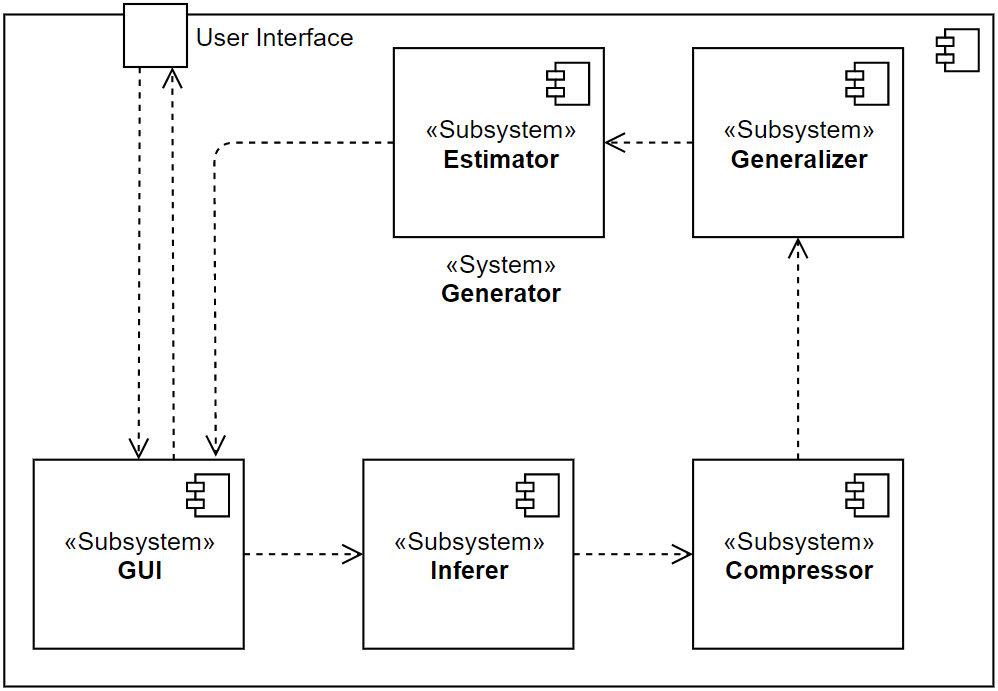
\includegraphics[width=12cm]{../images/Bausteinsicht_Ebene_1.PNG}
    \caption{Subsysteme mit fachlichen Abhängigkeiten}
\end{figure}

Betrachtet man die GUI-Komponente genauer, setzt sich diese aus vier Subsystemen zusammen.
Das Application-Modul beschreibt den Einstigspunkt für ein JavaFX-Programm.
Die grafische Benutzerschnittstelle wird über ein XML-basiertes FXML-Dateischema (Scene graph) mit zugeförigem FXML-Controller (Model)
aufgebaut.
Der Controller stellt die Logik für eine JavaFX-Oberfläche zur Verfügung.
Neben der Erstellung der Basisstruktur, wird die Baumstruktur in einer seperaten Komponente umgesetzt.

\underline{Ebene 2}
\begin{figure}[H]
    \centering
    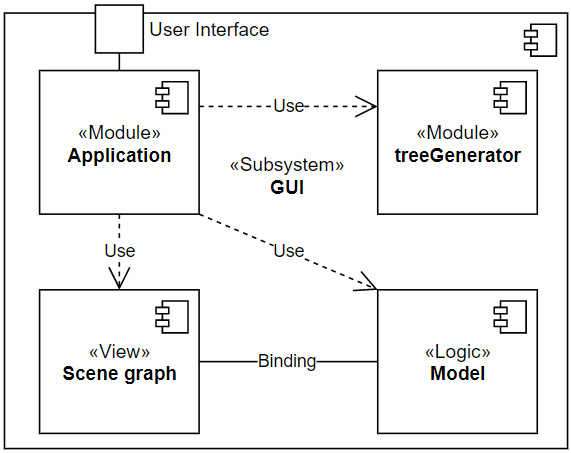
\includegraphics[width=9cm]{../images/Bausteinsicht_Ebene_2.PNG}
    \caption{Subsystem GUI}
\end{figure}

\subsection*{Laufzeitsicht}
Aus der nachfolgenden Abbildung geht hervor, wie sich der Informationsfluss zwischen den einzelnen Subsystemen verhält.
Wird der Systemprozess einmal durchlaufen, besteht die Möglichkeit die Ausführung des generalisierten L-Systems mit
erneuter Vergabe der Transformationsparameter aus der Häufigkeitsverteilung der Estimator-Komponente zu starten.
Der Ablauf des Systems setzt sich wie folgt zusammen:

\begin{figure}[H]
    \centering
    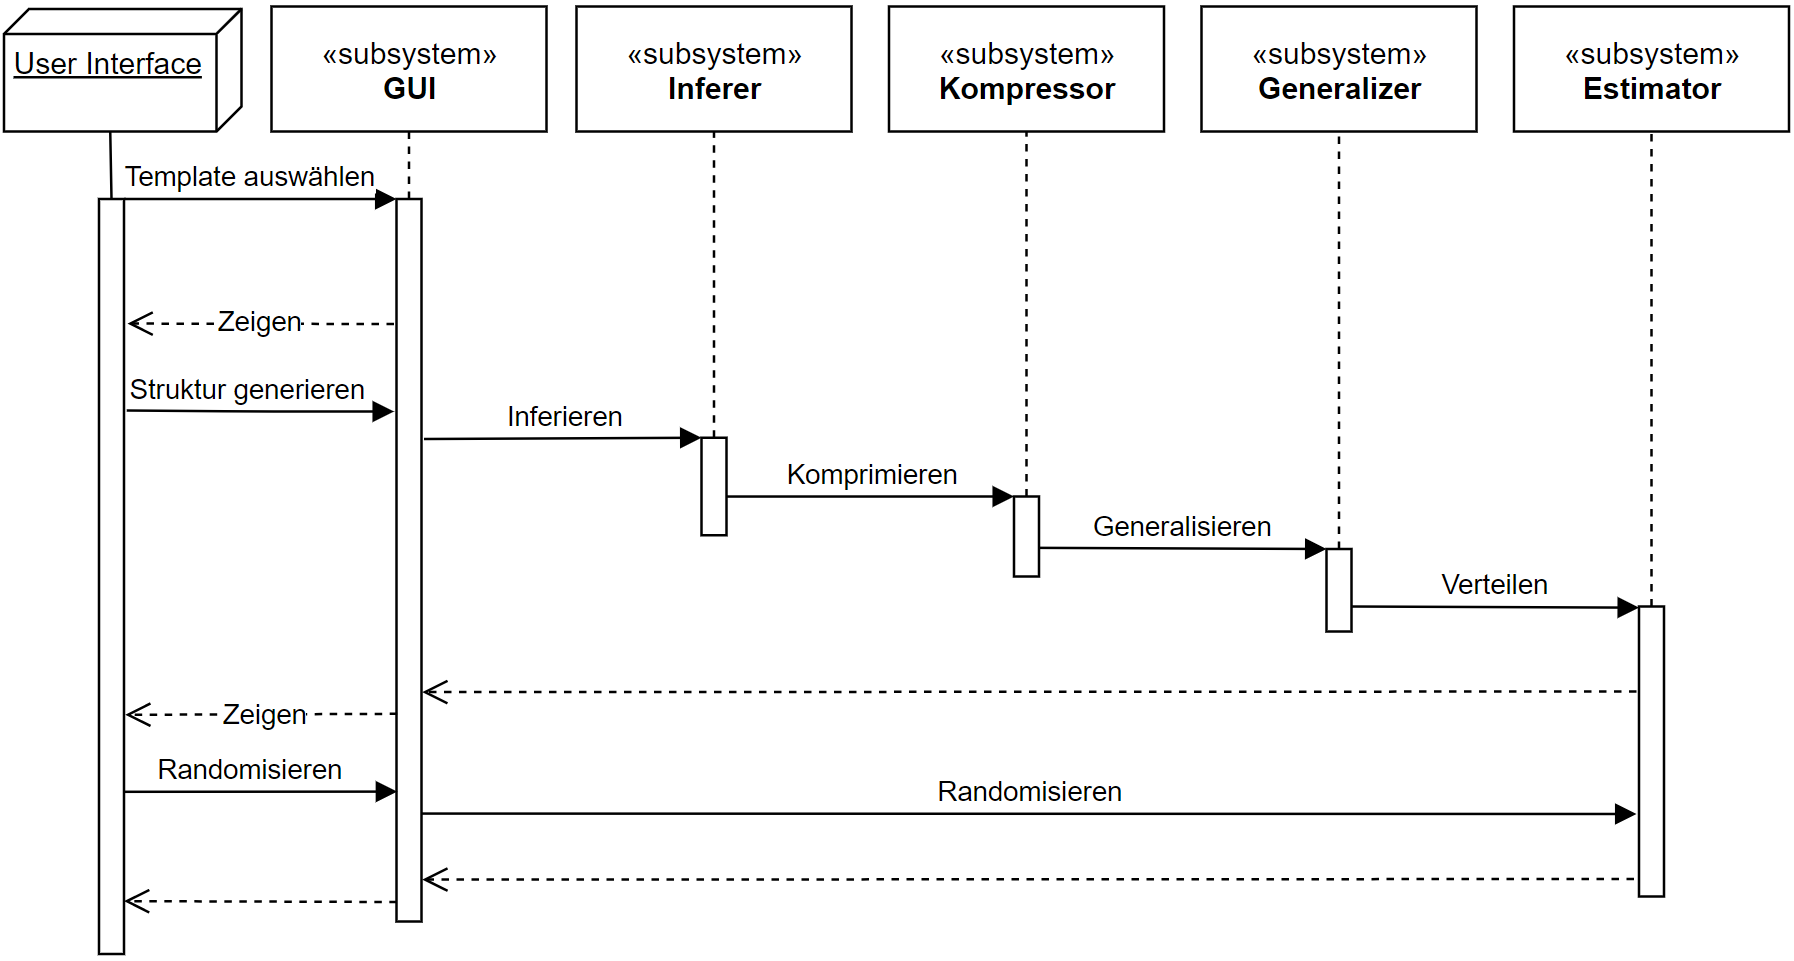
\includegraphics[width=14cm]{../images/Laufzeitsicht.PNG}
    \caption{Laufzeitsicht}
\end{figure}

\subsection*{Verteilungsicht}
Die Ausführung des Programms wird durch ein einfaches Startskript zur Verfügung gestellt.
Die folgende Abbildung der Verteilungssicht stellt lediglich die Ausführung auf einer Windows-Maschine dar.

\begin{figure}[H]
    \centering
    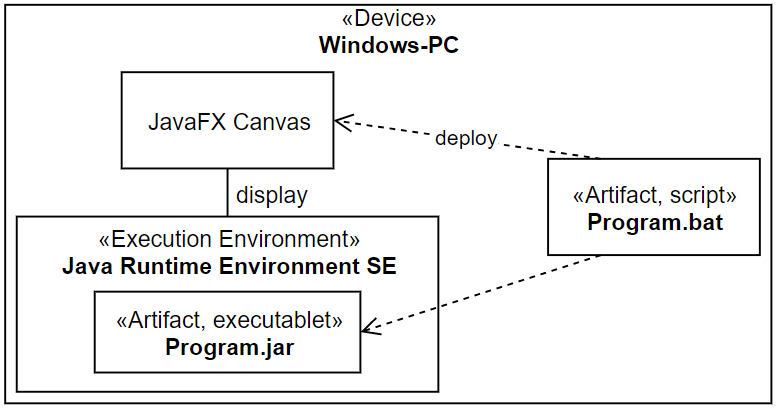
\includegraphics[width=10cm]{../images/Verteilungssicht.PNG}
    \caption{Infrastruktur Windows-PC}
\end{figure}

%\subsection{Weitere Konzepte}
%
%\subsubsection{Testbarkeit}
%Um eine ausreichende Testabdeckung zu erreichen, werden Klassen als kleinstmöglich zu testende Einheit definiert
%und durch Komponententests geprüft.
%Der Name eines Tests setzt sich aus dem Präfix als Name der zu testenden Klasse oder Releases und dem Suffix
%"`Test"'
%zusammen.
%Testsubjekte werden als \textbf{Blackbox} behandelt, also anhand der Spezifikation getestet.
%\begin{center}
%    Bsp.: Klasse \textit{Inferer} mit Komponententest \textit{InfererTest}
%\end{center}
%Da jedes Release der Implementierung ein funktionsfähiges System beinhaltet, kann auf Integrationstests
%verzichtet werden.
%Weiter wird ein Release anhand von funktionalen und nicht-funktionalen Anforderungen getestet.
%Anhand dieser Systemtests wird geprüft, ob Gesamtspezifikationen umgesetzt worden sind.
%\begin{center}
%    Bsp.: Release 2 mit Systemtest \textit{Release2Test}
%\end{center}
%Zum Schluss der Implementierung wird ein Akzeptanztest durchgeführt.
%
%\subsubsection{Validierung}
%Der Benutzer des Systems nutzt eine grafische Schnittstelle.
%Somit kann sichergestellt werden, dass dieser keine ungültigen Eingaben tätigt.
%Werden Template-Dateien unter einem bestimmten Dateipfad nicht gefunden, wird eine \textit{NotFound}-Exception
%protokolliert und dem Benutzer eine Nachricht über ein Pop-up mitgeteilt.
%Eine \textit{IllegalArgumentException} wird verzeichnet und ausgegeben, wenn eingelesene Template-Dateien
%strukturelle Fehler aufweisen.
%
%\subsubsection{Fehlerbehandlung}
%Zur Fehlersuche und -behandlung biete sich eine Protokollierung über Vorgänge, Fehler und Ausnahmen an.
%Bestimmte Fehler werden dem Benutzer weitergegeben und grafisch angezeigt.
%Folgende Subsysteme werden in das Programm integriert:
%\begin{itemize}
%    \item Ausnahmebehandlung (Exception Handling) und
%    \item Protokollierung (Logging)
%\end{itemize}
%Erwartete Exceptions werden jeweils mit eigenen Klassen abgebildet, die von einer entsprechenden Klasse aus der
%Exception-Hierarchie abgeleitet sind.
%Das Logging ist statisch und überall im System zugreifbar, um eine einheitliche Protokollierung zu gewährleisten.

\subsection*{Datenstrukturen}
Das Datenmodell ist als UML-Diagramm modelliert (siehe ~\ref{uml})